\documentclass[11pt,letterpaper]{article}
\usepackage[margin=1in]{geometry}
\usepackage[T1]{fontenc}
\usepackage{amsmath,amssymb}
\usepackage{booktabs}
\usepackage{graphicx}
\usepackage{enumitem}
\usepackage[hidelinks]{hyperref}
\setlist[itemize]{nosep,topsep=4pt}

\title{Multiple-Impulse Spacecraft Rendezvous Optimization}
\author{Hasnain}
\date{\today}

% Replace the prompts with your own writing as the report develops.
% Include only experiments and checks actually performed.
% This outline is a suggested structure, not an assessment rubric.
\newcommand{\prompt}[1]{\par\noindent\textit{Writing prompt:} #1\par}
\newcommand{\abs}[1]{\left\lvert#1\right\rvert}

\begin{document}
\maketitle

\begin{abstract}
\prompt{Write this last. In one paragraph, state the rendezvous problem,
the model and search method used, the main quantitative result, and the
most important conclusion or limitation. Leave results unspecified until
you have verified them.}
\end{abstract}

\section{Introduction and Aim}
\subsection{Spacecraft Trajectory Optimization Problem}
This problem discusses how a spacecraft in a distnct orbit from another object in an orbit can rendezvous at a specific location in space at a particular time
with the same velocity while minimizing the amount of fuel usage. For this specific project, we will be focusing on 2 spacecrafts in orbit around Earth where one
is defined as the \textit{chaser} spacecraft and the other is the \textit{target} spacecraft. % Requires a citation for the project outline provided by Mingde intext here

\subsection{Project Aim and Research Question} % This section as a whole should be cited with Mingde's project outline as he is the one who defined these things for me
This leads us to the question that I aim to work around:
\begin{center}
How can a spacecraft use a small number of engine burns to rendezvous with another spacecraft orbiting Earth?
\end{center} % This needs a citation for the project outline provided by Mingde
Thus, the aim of this project that follows is to develop a simulator for orbital rendezvous missions. I will begin with a simplified model in 2 dimenions
and only considering the Earth as the only relevant gravitational body. I will look to minimize the following 2 errors:

Position Error:
\begin{equation}
J_r = \abs{r_c(T) - r_t(T)}^2
\label{eq:postion_error}
\end{equation}

Velocity Error: 
\begin{equation}
J_v = \abs{v_c(T) - v_t(T)}^2
\label{eq:velocity_error}
\end{equation}

In addition to position and velocity error, I will be taking into account fuel usage with the assumption that fuel usage is directly proportional to the change in velocity
in the $x$, $y$, and $z$ directions. These three will be combined into the following cost function:

\begin{equation}
J = \omega_{r}J_{r} + \omega_{v}J_{v} + \omega_{\Delta v}\sum_{i} \abs{\Delta v_i}
\label{eq:cost_function}
\end{equation}

After testing with the 2 dimensional model, the aim will be to expand to 3 dimensions and will consider the Moon, Sun and Jupiter as
gravitationally relevant bodies to the motion of the spacecrafts.

\section{Physical Model and Problem Definition}
\subsection{Assumptions and equations of motion}
To begin, the following assumptions will be used for the 2 dimensional model
\begin{itemize}
  \item Planar motion in an Earth-centred inertial Cartesian frame.
  \item Central gravity with constant gravitational parameter $\mu$.
  \item An uncontrolled target and a chaser with instantaneous burns.
  \item Fuel usage is directly proportional to change in velocity of a burn.
\end{itemize}
For each spacecraft, position is defined as $\mathbf r=\begin{bmatrix} x \\ y \end{bmatrix}$ and velocity is defined as $\mathbf v=\begin{bmatrix} v_x \\ v_y \end{bmatrix}$:
\begin{equation}
  \dot{\mathbf r}=\mathbf v,
  \qquad \dot{\mathbf v}=-\mu\frac{\mathbf r}{\|\mathbf r\|^3}.
  \label{eq:ODE}
\end{equation}
Equation~\eqref{eq:ODE} defines the ODE that the spacecraft states will be modelled after, with $\mu$ defined as the gravitational parameter and for the 2 dimensional model
is the gravitational parameter of Earth:
\begin{align*}
  \mu&=GM\\
  \mu&=3.986\times10^{14}
\end{align*}
At burn time $t_i$, position is continuous and velocity changes according to
\begin{equation}
  \mathbf v(t_i^+)=\mathbf v(t_i^-)+\Delta\mathbf v_i.
  \label{eq:instantaneous_burns}
\end{equation}
Equation~\eqref{eq:instantaneous_burns} is the mathematical representation of the assumption that all burns are applied as instantaneous burns, meaning that position does
not change but the velocity changes instantly right after time $t_i$. 

For the three-dimensional model, the assumptions are extended as follows:
\begin{itemize}
  \item Three-dimensional motion in a Sun-centred Cartesian frame, treated
        as inertial under the approximation that the Sun is physically
        fixed at the origin with zero velocity.
  \item Newtonian point-mass gravity from the Sun, Earth, Moon, and Jupiter,
        each with a constant gravitational parameter $\mu_b$.
        Earth, the Moon and Jupiter move under the gravity of all four bodies.
        The Sun attracts the moving bodies but does not respond to their
        gravitational attraction.
        Spacecraft masses are negligible, and other gravitational bodies
        and non-gravitational forces are neglected.
  \item An uncontrolled target and a chaser with instantaneous burns.
        Position remains continuous across each burn, while velocity
        changes instantaneously.
  \item Total impulse magnitude,
        $\sum_i \|\Delta\mathbf v_i\|$,
        is used as a proxy for propellant consumption and is part of the third term for Equation~\ref{eq:cost_function}, the cost function.
\end{itemize}
\subsection{Scenario and definition of success}
We can begin with defining the initial state of a spacecraft using the position and velocity vectors in 2 dimensions as follows:
\begin{equation}
  \mathbf{\vec{v}}=\begin{bmatrix} x \\ y \\ v_x \\ v_y \end{bmatrix}
  \label{eq:initial_2D_state}
\end{equation}
Then applying ODE in Equation~\ref{eq:ODE} to the derivative of the initial state, we obtain:
\begin{equation}
  \mathbf{\vec{v'}}=\begin{bmatrix} v_x \\ v_y \\ a_x \\ a_y \end{bmatrix}
  \label{eq:initial_2D_state_derivative}
\end{equation}
\begin{equation}
  \mathbf{\vec{v'}}=\begin{bmatrix} v_x \\ v_y \\ -\mu\frac{x}{\abs{r}^3} \\ -\mu\frac{y}{\abs{r}^3} \end{bmatrix}
  \label{eq:initial_2D_state_derivative_ODE}
\end{equation}
Then with any final time $T$, the number of burns and the initial state of both spacecrafts defined as shown in Equation~\ref{eq:initial_2D_state}
the rendezvous between the \textit{chaser} and \textit{target} spacecraft can be determined.

For the initial state of the 3 dimensional model with more than one significant gravitational body, we can define the acceleration using the same base ODE
from Equation~\ref{eq:ODE}, but make the following changes to the original model:
\begin{align}
  \ddot{\mathbf r}&=-\mu\frac{\mathbf r}{\|\mathbf r\|^3}.\notag\\
    \ddot{\mathbf r}&=\sum_{i=0}^{n-1}-\mu_i\frac{r_i}{\abs{r_i}^3}
    \label{eq:3D_ODE}
\end{align}
Here, $n$ is the number of gravitational bodies being considered, and where $\mu_i$ and $r_i$ correspond to the i-th gravitational body on a 0 index.
For my case, the gravitational bodies will be defined as follows:

\[[\text{Sun}, \text{Earth}, \text{Moon}, \text{Jupiter}]\]

The following gravitational parameters, $\mu$ will be used for the gravitational bodies:
\begin{center}
  \begin{tabular}{lc}
    \toprule
    Body & $\mu$ ($\mathrm{m^3\,s^{-2}}$) \\
    \midrule
    Sun     & $1.3271\times10^{20}$ \\
    Earth   & $3.986\times10^{14}$ \\
    Moon    & $4.9028\times10^{12}$ \\
    Jupiter & $1.2671\times10^{17}$ \\
    \bottomrule
  \end{tabular}
\end{center}

Furthermore, we will define a successful rendezvous as follows:
\begin{itemize}
  \item $\text{Final Separation}<=1000 m$
  \item $\text{Velocity Difference}<=1 ms^{-1}$
\end{itemize}
Final docking and approach are not within the scope of the project so this is sufficient for a successful rendezvous

\section{Computational Method}
\subsection{Trajectory propagation}
To begin, I use Python to calculate how the initial states of both spacecrafts
change over time. The equations of motion are solved using the
\texttt{solve\_ivp} function from SciPy, with the \texttt{DOP853} method.
This method adjusts the size of its time steps as the trajectory is
calculated. For both models, I set the relative tolerance to $10^{-6}$
and leave the absolute tolerance at its default value of $10^{-6}$.
These tolerances control the numerical integration error; they do not
directly define the final separation required for a successful rendezvous.

\subsubsection{Two-dimensional model}
For the original 2 dimensional model, the initial states are entered in
the form shown in Equation~\ref{eq:initial_2D_state}, with positions in
metres and velocities in metres per second relative to the fixed Earth.
The final time $T$ and number of burns are also specified before the
search begins. The target is first propagated from $t=0$ to $t=T$ without
any burns. I keep a continuous interpolated solution of its state using
\texttt{dense\_output}, allowing its position and velocity to be obtained
at any time within the simulation. This target solution is reused when
testing different burn sequences, since the chaser's burns do not affect
the target's motion.

For the chaser, the trajectory is divided into intervals separated by
the burn times. The ODE is first solved from the initial time to the
first burn. At that time, the change in velocity is added to the state
while position remains unchanged, as described in
Equation~\ref{eq:instantaneous_burns}. The updated state is then used as
the initial state for the next interval. This process is repeated for
each burn, followed by a final propagation to $T$. Thus, both spacecrafts
are compared at the same final time even though the chaser's motion is
calculated in separate intervals.

\subsubsection{Three-dimensional model with multiple gravitational bodies}
For the 3 dimensional model, the initial spacecraft states contain six
values, $[x,y,z,v_x,v_y,v_z]$. I first obtain the initial states of Earth,
the Moon and Jupiter from JPL Horizons, using the default starting epoch
of 27 October 2026 at 12:00:00 UTC. These values are converted
from kilometres and kilometres per second to SI
units. The Sun is fixed at the origin with zero velocity throughout
the simulation.

Earth, the Moon and Jupiter are then propagated under their mutual
gravitational attraction and the Sun's gravity. I keep the same combined
state of 24 values, with six values for each body, but set all six
derivatives of the Sun's state to zero. This calculation is performed once before
the rendezvous search, using the same solver and tolerances as the
spacecraft propagation. A continuous interpolated solution is retained
so that the location of each body can be obtained at the times requested
by the spacecraft solver. I chose to hold the Sun fixed to simplify the model by
neglecting its response to the other bodies.

The spacecraft states entered into the simulator describe their initial
positions and velocities relative to Earth. I add Earth's initial
position and velocity so that the spacecrafts and gravitational bodies
can be tracked together with the Sun at the origin. At each time, I
calculate the distance and direction from each body to the spacecraft
and add the four gravitational contributions to obtain its acceleration:
\begin{equation}
  \mathbf a(t)=-\sum_{b=1}^{4}\mu_b
  \frac{\mathbf r(t)-\mathbf r_b(t)}
       {\|\mathbf r(t)-\mathbf r_b(t)\|^3},
  \label{eq:computed_3D_acceleration}
\end{equation}
where $\mathbf r(t)$ and $\mathbf r_b(t)$ are the positions of the
spacecraft and gravitational body $b$, respectively, measured from
the Sun. Their difference gives the spacecraft's displacement from that
body. The target is propagated once for the search, and the chaser is
propagated between burns in the same way as the 2 dimensional model.
Both spacecrafts use the same precomputed body trajectories. Their
masses are neglected, so neither spacecraft changes the motion of the
four bodies or the other spacecraft.

\subsection{Burn representation}
In both implementations, a burn is stored as a pair $(d_i,t_i)$, where
$d_i$ is a signed burn magnitude and $t_i$ is the time of the burn.
To simplify the search, burns are restricted to act along or opposite
to the chaser's motion relative to Earth just before the burn. The
resulting velocity change is added to the chaser's velocity, while its
position remains unchanged. This is expressed as follows:
\begin{equation}
  \Delta\mathbf v_i=d_i
  \frac{\mathbf v_{c/E}(t_i^-)}{\|\mathbf v_{c/E}(t_i^-)\|}.
  \label{eq:computed_burn_direction}
\end{equation}
A positive value of $d_i$ applies the burn along this velocity, while a
negative value applies it in the opposite direction. Thus, each burn
has two search variables rather than separate velocity changes in
each coordinate direction.

For the 2 dimensional model, Earth is fixed, so
$\mathbf v_{c/E}=\mathbf v_c$. For the 3 dimensional model, I obtain
Earth's velocity from the precomputed body solution at each burn time
and subtract it from the chaser's velocity:
\begin{equation}
  \mathbf v_{c/E}(t_i^-)=\mathbf v_c(t_i^-)-\mathbf v_E(t_i).
\end{equation}
This gives the direction of the spacecraft's motion relative to Earth
at the time of the burn. The same calculation is used when scoring candidate sequences
and when reconstructing the selected trajectory for plotting.

\subsection{Objective function and search}
After each candidate burn sequence has been propagated, I calculate
the squared position and velocity differences at $T$. The total change
in velocity is calculated by adding the absolute values of the signed
burn magnitudes:
\begin{equation}
  \Delta v_{\mathrm{total}}=\sum_{i=1}^{N}|d_i|
  =\sum_{i=1}^{N}\|\Delta\mathbf v_i\|.
\end{equation}
These three quantities are combined using the cost function defined in
Equation~\eqref{eq:cost_function} to score each candidate burn sequence.
The weights determine how much each term contributes to the search.
This scaling is necessary because position error, velocity error and
total change in velocity have different units and numerical sizes.
For the original 2 dimensional script, the weights are fixed as
\begin{equation}
  (\omega_r,\omega_v,\omega_{\Delta v})
  =(10^{-8},10^{-2},10^{-3}),
\end{equation}
when the states and burns are expressed in SI units. In the
3 dimensional script, the three positive weights are supplied when
running the program, allowing different choices to be tested.

To search for a burn sequence, I use SciPy's
\texttt{differential\_evolution} function. This method starts with a
population of candidate sequences, generates new candidates by
combining and changing their parameter values, and keeps candidates
with lower costs. For $N$ burns, there are $2N$ parameters to search.
The burn magnitude limits are $500\ \mathrm{m\,s^{-1}}$ for the original
2 dimensional model and $1000\ \mathrm{m\,s^{-1}}$ for the 3 dimensional
model. Thus, for the 3 dimensional search, the bounds are
\begin{align}
  -1000\ \mathrm{m\,s^{-1}} &\leq d_i\leq1000\ \mathrm{m\,s^{-1}},\\
  60\ \mathrm{s} &\leq t_i\leq T-60\ \mathrm{s}.
\end{align}
The burn times must be strictly increasing. A candidate with repeated,
out-of-order or out-of-interval burn times is assigned a cost of
$\infty$ before propagation. The 60 second margin applies at the
beginning and end of the mission; it is not a minimum spacing between
successive burns. No collision-avoidance constraint is included in
these scoring functions.

Both scripts use a random seed of 42 and leave the remaining optimizer
settings at the SciPy defaults. In the installed SciPy version 1.17.1,
these include the \texttt{best1bin} strategy, a population size of
$15(2N)=30N$, and a maximum of 1000 generations. The search can stop
earlier when the spread of population costs meets the default
convergence tolerance of 0.01, with zero absolute tolerance. A final
local polishing step is enabled by default. The returned sequence is
therefore the best sequence found by this search, rather than a
guaranteed global minimum. The previously defined final separation
and velocity criteria must still be checked separately; they are not
enforced as constraints by the optimizer.

\subsection{Trajectory reconstruction and visualization}
Once a sequence has been selected, I propagate it again to produce the
trajectory plots. By default, the chaser is sampled at 1000 equally
spaced output times per interval, and repeated interval endpoints are
removed when joining the histories. These output times are used for
plotting and do not force the ODE solver to use a fixed integration
step. The target's continuous solution is evaluated at the chaser's
sample times to calculate their separation.

For the 2 dimensional model, the plots show the trajectories around
Earth and the separation over time, with the burn locations marked.
For the 3 dimensional model, the plots include separation over time
and both a view of the system around the Sun and a close-up of the
rendezvous around Earth. For the Earth close-up, I subtract Earth's
position from each spacecraft's position at the same time. This makes
the motion around Earth easier to see without changing the calculated
trajectories or burn directions.

\section{Simulation Checks}
The implementation was checked using 28 automated tests, all of which
passed. These checks are described in Appendix~\ref{app:implementation_checks}.
The following checks focus on the numerical accuracy of the simulated
motion and the reported rendezvous results.

\subsection{Circular-orbit reference case}
For the 2 dimensional model, I tested a circular orbit with a radius of
$7.0\times10^6\ \mathrm{m}$ and an initial speed of
$\sqrt{\mu/r}$. I propagated the spacecraft for one orbital period,
approximately $5828.52\ \mathrm{s}$, using the setting defined for \texttt{solve\_ivp} in the previous section.
The simulated position was compared with the analytical circular motion
at 1000 output times. The maximum position difference was $18.94\ \mathrm{m}$,
and the difference after one full orbit was $15.97\ \mathrm{m}$.
The maximum relative changes in specific orbital energy and angular
momentum were $2.12\times10^{-6}$ and $1.06\times10^{-6}$, respectively.
This provides a reference check for the original Earth-only model.

\subsection{Sensitivity to numerical tolerances}
The solver calculates an approximation of the spacecraft motion.
I therefore checked whether using lower numerical tolerances would
significantly change the simulated results, particularly whether
attempts previously classified as successful or unsuccessful would
change classification. This check was performed for the 3 dimensional
model, but the same procedure can also be applied to the 2 dimensional
model.

The validation experiments in Section 5 tested four sets of weights
on eight retained initial-state cases, giving 32 burn sequences in the
reported dataset. I simulated all 32 sequences again with tighter numerical tolerances, which require
the solver to control its calculation error more closely. The burn
times and magnitudes stayed the same; only the accuracy settings
changed. The gravitational-body motion was also recalculated with
the tighter settings. The settings are listed in Appendix A.

In the original simulations, two of the 32 retained attempts finished within
1000 m of the target with a relative speed no greater than
$1\ \mathrm{m\,s^{-1}}$. The lower tolerances gave the same
two passes and 30 failures. I then simulated the two passing sequences
once more with a still lower relative tolerance, and both continued to pass.

The calculated distances did change, even though the success results
did not. Table~\ref{tab:tolerance_checks} shows both passing
attempts from this final check, all using the overall-winning weights. For the 1 km initial
offset, the final separation changed from approximately 16 m to 75 m.
Both values are below the 1000 m limit defined earlier. Thus, lowering
the tolerances changed some calculated final distances but did not
change which of the tested attempts met the rendezvous criterion.

I also wanted to assess whether the additional accuracy would justify
the extra computation required by lower tolerances. However, runtime
was not measured, so the trade-off between accuracy and computation
time was not quantified. For stricter rendezvous requirements, lower
tolerances may be necessary to keep numerical errors small enough
to assess success reliably.

\begin{table}[htbp]
\centering
\caption{Original results and the final, tighter-tolerance check for the two
successful attempts using the overall-winning weights. Burn times and
magnitudes are unchanged.}
\label{tab:tolerance_checks}
\begin{tabular}{lrrrr}
\toprule
Initial case & \multicolumn{2}{c}{Original} & \multicolumn{2}{c}{Tighter check}\\
 & $e_r$ (m) & $e_v$ (m/s) & $e_r$ (m) & $e_v$ (m/s)\\
\midrule
1 km along-track & 16.0 & 0.037 & 74.6 & 0.039\\
10 km along-track & 149.5 & 0.251 & 172.8 & 0.243\\
\bottomrule
\end{tabular}
\end{table}

\section{Experiments and Results}
\subsection{Experiment setup and weight selection}
For these experiments, I used the 3 dimensional model with the Sun fixed
at the origin and Earth, the Moon and Jupiter moving under gravity.
The mission duration was $3600\ \mathrm{s}$, with two burns bounded
between $-1000$ and $1000\ \mathrm{m\,s^{-1}}$ each. The saved initial
body states, solver settings and optimizer seed of 42 were reused
throughout the sweep and validation. Earlier experiments with different
burn directions or magnitude limits were kept separate.

The initial state used to select the weights was
\begin{align*}
\text{Chaser: } &[7000000,-500000,300000,0,7400,500],\\
\text{Target: } &[7000000,0,0,0,7546,0],
\end{align*}
where the entries are $[x,y,z,v_x,v_y,v_z]$ relative to Earth, in metres
and metres per second. The initial search tested 1000 weight combinations,
with each of the three weights taking one of 10 values from 0.001 to 1,000,000,
increasing by a factor of 10 between values. Then 312 additional refined combinations
were tested within a smaller range. In the end, all 1312 trials returned finite
results with valid burns and passed the sampled surface check. This
status does not mean that they achieved rendezvous.

To compare results obtained with different weights, I used a similar
dimensionless comparison score for every trial:

\begin{equation}
S=\left(\frac{e_r}{100\ \mathrm{m}}\right)^2
 +\left(\frac{e_v}{0.1\ \mathrm{m\,s^{-1}}}\right)^2
 +\frac{\Delta v_{\mathrm{total}}}{500\ \mathrm{m\,s^{-1}}}.
\end{equation}

Here, $e_r$ and $e_v$ are the final separation and relative speed from each trial.
The raw cost values from differently weighted objectives were not used to rank
different weight tuples directly. This comparison score essentially makes all three
values being measured for cost have the same impact.

I selected four weight tuples from the sweep: the lowest comparison
score overall, the lowest comparison score from the first 1000 comparisons, the
lowest final position error, and the lowest final velocity error.
These weights were saved before testing the additional initial states.
Table~\ref{tab:selected_weights} lists the selected values and their
subsequent validation results.

\begin{table}[htbp]
\centering
\caption{Selected weights and project-criterion passes across the seven
new initial states. The original selection case is excluded from the counts.}
\label{tab:selected_weights}
\begin{tabular}{lrrrr}
\toprule
Selection & $\omega_r$ & $\omega_v$ & $\omega_{\Delta v}$ & Passes\\
\midrule
Overall (All 1312) & 0.0075 & 5000 & 2.5 & 2/7\\
First 1000 & 0.001 & 10000 & 10 & 0/7\\
Position & 1 & 0.1 & 1 & 0/7\\
Velocity & 0.005 & 75000 & 2.5 & 0/7\\
\bottomrule
\end{tabular}
\end{table}

\subsection{Results for the original selection case}
Table~\ref{tab:selection_case} compares the four selected weight tuples
on the original initial states. None met the project rendezvous criterion.
The overall-winning sequence applied a $+984.30\ \mathrm{m\,s^{-1}}$
burn at $61.67\ \mathrm{s}$ and a $-900.70\ \mathrm{m\,s^{-1}}$ burn
at $354.19\ \mathrm{s}$. Its minimum sampled separation was approximately
24.38 km during the trajectory, but it finished approximately 563.50 km
from the target. Thus, its closest approach was not a terminal rendezvous.

The no-burn trajectory for this initial state entered Earth's sampled
surface. Its final separation was approximately 2493.54 km and its
relative speed was $2114.99\ \mathrm{m\,s^{-1}}$, but these terminal
values come from continuing the point-mass simulation after surface
intersection. They do not describe a physically flyable coast trajectory.

\begin{table}[htbp]
\centering
\caption{Results for the original weight-selection experiment.}
\label{tab:selection_case}
\begin{tabular}{lrrr}
\toprule
Selection & Final separation (km) & Relative speed (m/s) & Total $\Delta v$ (m/s)\\
\midrule
Overall (1312) & 563.50 & 134.36 & 1885.00\\
First 1000 & 563.77 & 133.95 & 1898.36\\
Position & 563.39 & 390.53 & 1222.83\\
Velocity & 564.49 & 133.90 & 1662.79\\
\bottomrule
\end{tabular}
\end{table}

\subsection{Validation on different initial states}
The validation analysis includes the four selected weight tuples on the original case
and seven new cases, giving 32 powered optimization trials. For
each of the eight retained initial-state cases, I also simulated the spacecraft
motion without any burns to create a baseline to compare the final results
to. For each combination of weights and initial states, I searched for new
burn times and magnitudes.

The new cases included along-track offsets of 1 km and 10 km,
a radial offset, a cross-track offset, a mixed position and velocity
offset, a higher target orbit, and an inclined target orbit. The full
initial states, weights, selected burns and measurements are recorded
in Appendix~\ref{app:validation_data}. Table~\ref{tab:new_cases} shows
the production results for the overall-winning weights, and
Figure~\ref{fig:validation_comparison} compares their final errors
with the no-burn controls.

\begin{table}[htbp]
\centering
\caption{Production validation results using the overall-winning weights.
A pass requires both $e_r\leq1000$ m and $e_v\leq1$ m/s.}
\label{tab:new_cases}
\begin{tabular}{lrrrl}
\toprule
Case & $e_r$ (m) & $e_v$ (m/s) & Total $\Delta v$ (m/s) & Pass\\
\midrule
1 km along-track & 16.0 & 0.037 & 6.30 & Yes\\
10 km along-track & 149.5 & 0.251 & 101.50 & Yes\\
10 km radial & 2871.1 & 5.224 & 372.01 & No\\
10 km cross-track & 13639.8 & 0.340 & 18.89 & No\\
Mixed, about 100 km & 41209.7 & 3.272 & 151.45 & No\\
Higher target orbit & 2086.6 & 1.972 & 34.99 & No\\
Inclined target orbit & 6166.4 & 1.216 & 758.70 & No\\
\bottomrule
\end{tabular}
\end{table}

Figure~\ref{fig:successful_trajectories} shows the two successful
attempts using the overall-winning weights. The orbit views show
their motion around Earth, while the close-ups show the chaser's
position relative to the target. The paths nearly overlap at the
scale of the orbit, so the close-ups make their separation easier
to see.

\begin{figure}[p]
\centering
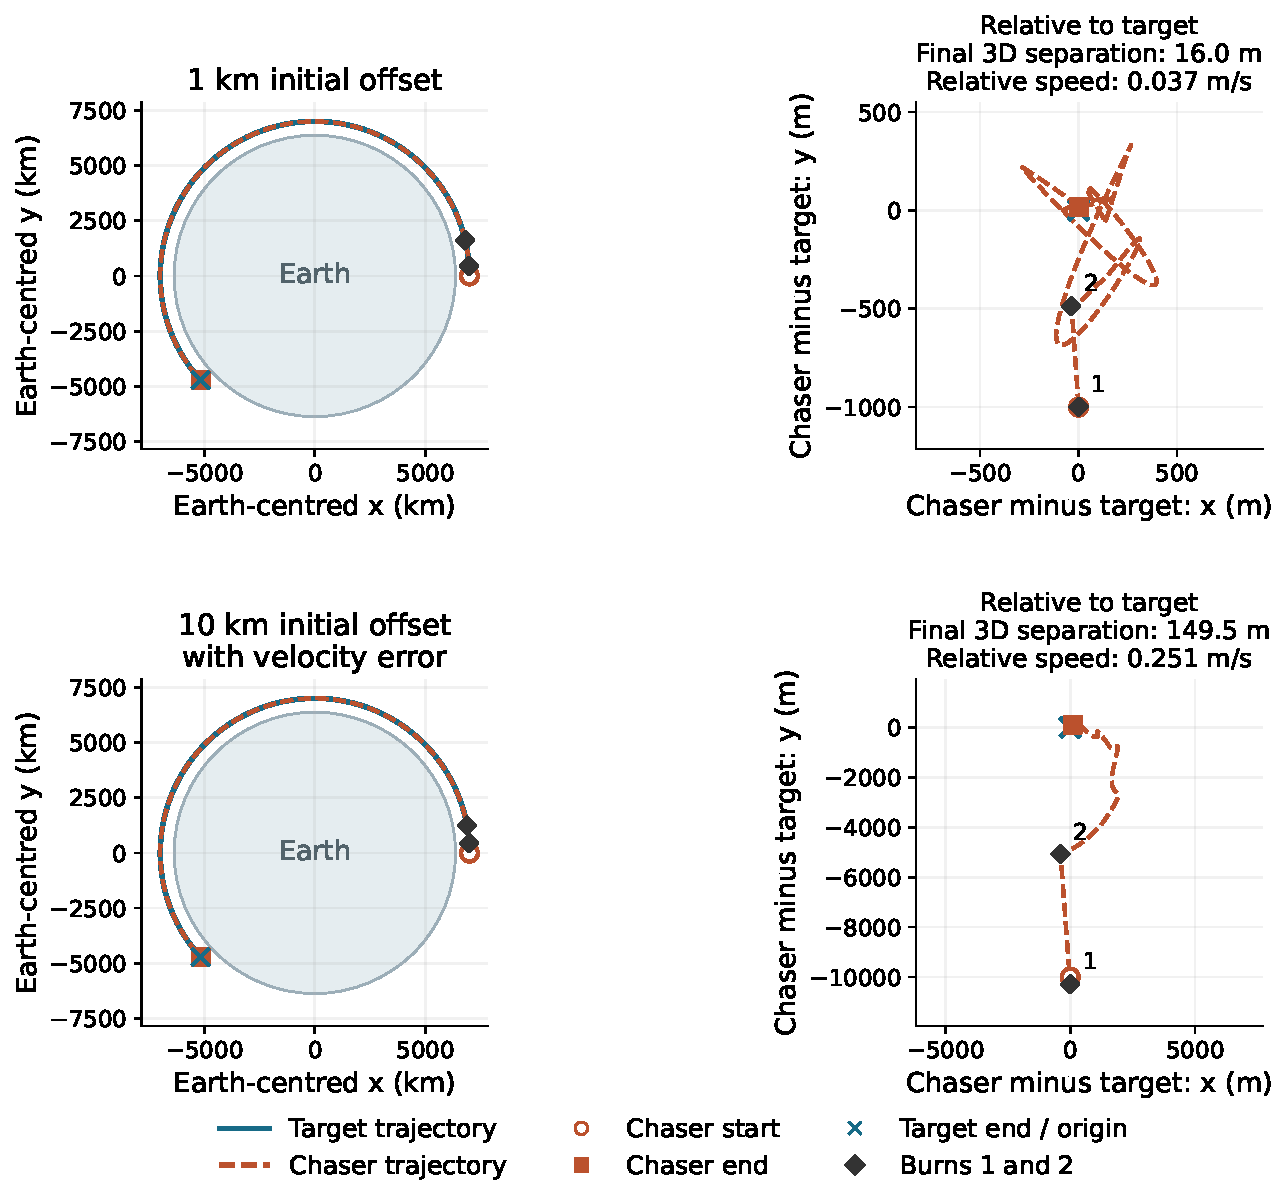
\includegraphics[width=\linewidth,height=0.78\textheight,keepaspectratio]{outputs/weight_validation_fixed_sun_20261029_144240/report_successful_trajectories.pdf}
\caption{Successful validation attempts using the overall-winning weights.
Each row shows an Earth-centred orbit view (left) and the chaser's
motion relative to the target (right). Both views are $x$--$y$
projections of the 3 dimensional trajectories; the final separation
and relative speed use all three components. Numbered diamonds in
the close-ups mark the two burns. The target is at the origin in
each close-up.}
\label{fig:successful_trajectories}
\end{figure}

\begin{figure}[htbp]
\centering
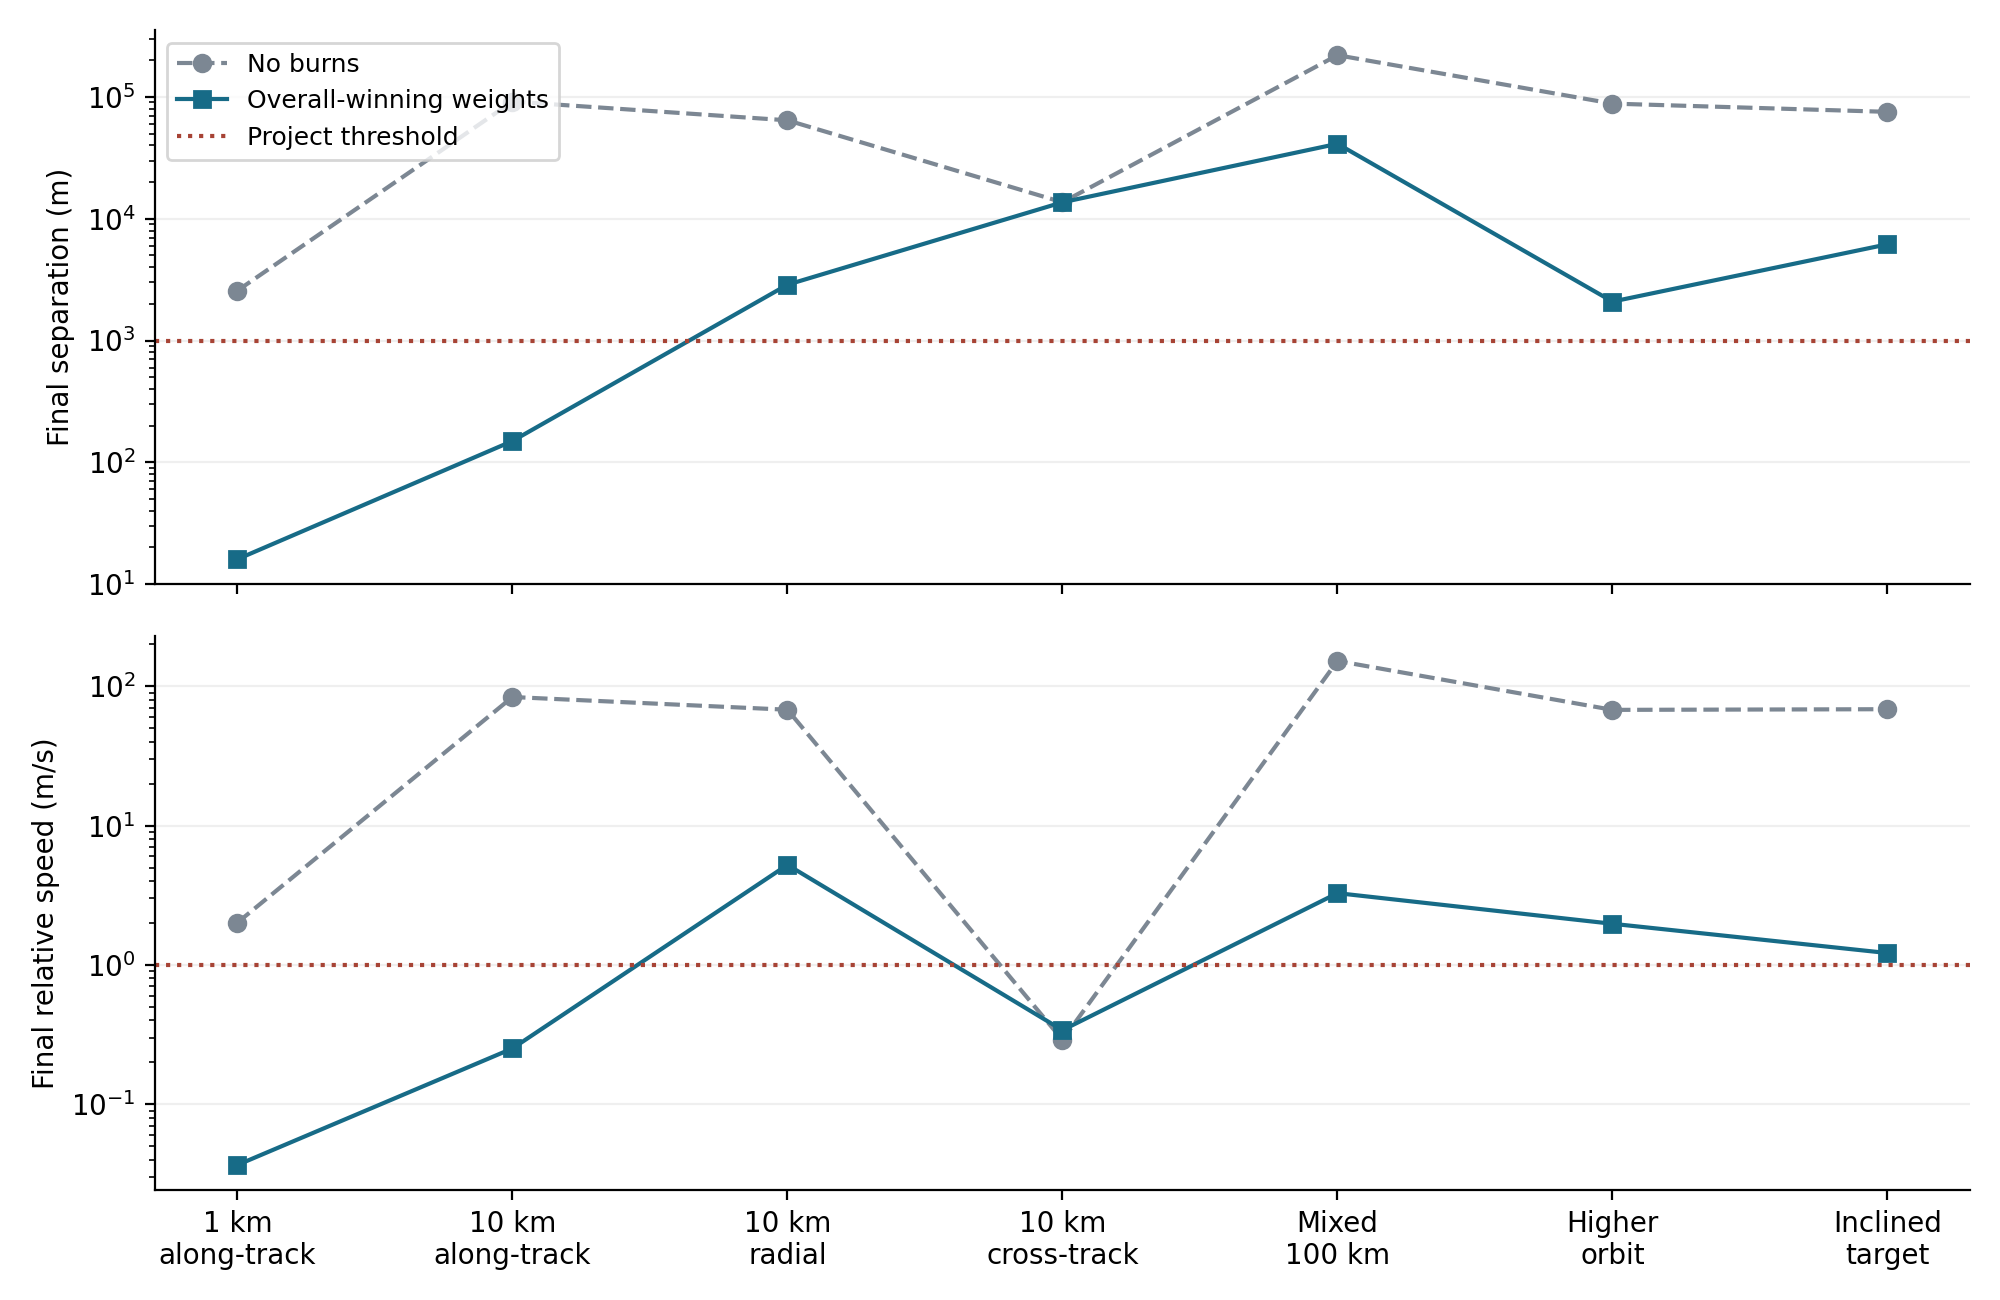
\includegraphics[width=\linewidth]{outputs/weight_validation_fixed_sun_20261029_144240/report_validation.png}
\caption{Final separation and relative speed for the seven new
cases, comparing the overall-winning weights with no burns. The vertical
scales are logarithmic; dotted lines show the project thresholds.}
\label{fig:validation_comparison}
\end{figure}

The overall-winning weights also achieved rendezvous in the 1 km
and 10 km along-track cases, whereas both no-burn baselines failed.
For the 1 km case, the optimized burns reduced the final separation
from 2568.4 m to 16.0 m and the relative speed from
$2.011\ \mathrm{m\,s^{-1}}$ to $0.037\ \mathrm{m\,s^{-1}}$.
For the 10 km case, they reduced the final separation from 91560.0 m
to 149.5 m and the relative speed from $83.754\ \mathrm{m\,s^{-1}}$
to $0.251\ \mathrm{m\,s^{-1}}$.

For the successful 1 km case, the selected burns were
$+3.127\ \mathrm{m\,s^{-1}}$ at $60.014\ \mathrm{s}$ and
$-3.173\ \mathrm{m\,s^{-1}}$ at $216.811\ \mathrm{s}$.
Figure~\ref{fig:successful_history} shows its separation and relative
speed over the mission. The lower-tolerance recheck in
Table~\ref{tab:tolerance_checks} also met the secondary, stricter
criterion of 100 m and $0.1\ \mathrm{m\,s^{-1}}$.

\begin{figure}[htbp]
\centering
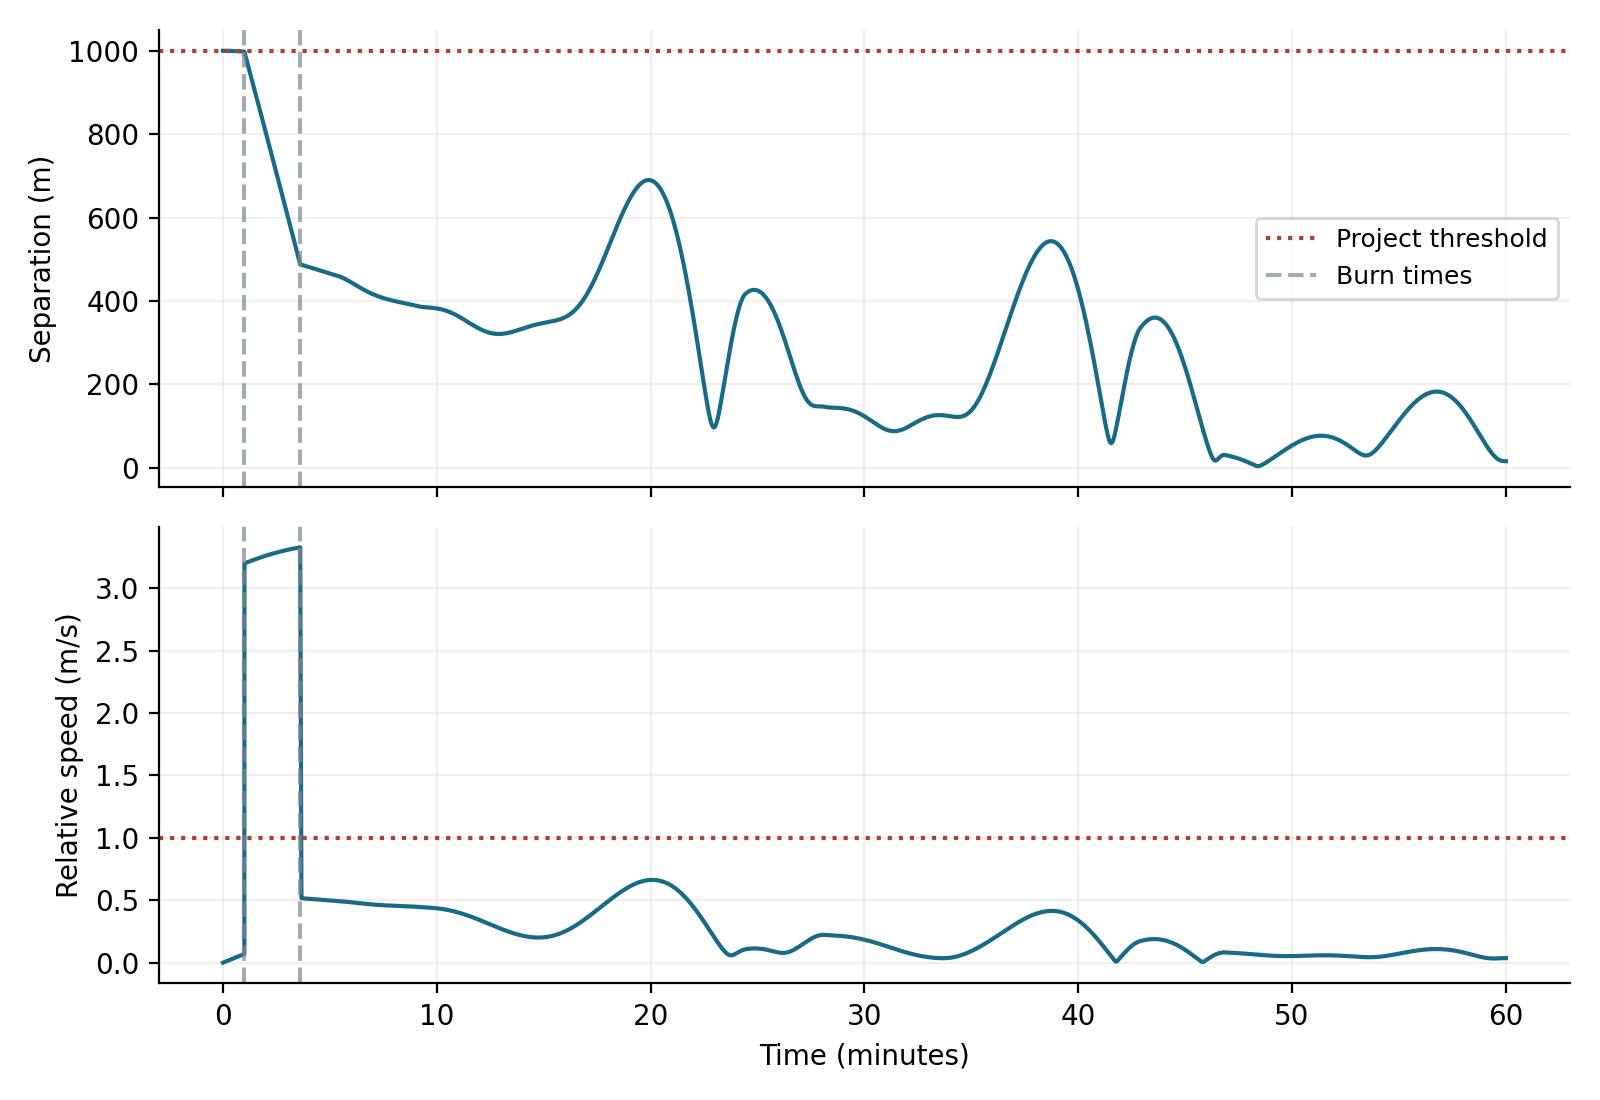
\includegraphics[width=0.9\linewidth]{outputs/weight_validation_fixed_sun_20261029_144240/report_success_history.png}
\caption{Production separation and relative speed for the 1 km along-track
case using the overall-winning weights. Dashed lines mark the two burns;
dotted lines show the project success thresholds.}
\label{fig:successful_history}
\end{figure}

Across the seven new states, the best weights from the initial 1000
combinations, the position selection and the velocity selection all
failed to meet the rendezvous criterion. As an
example of the difference between matching position and achieving
rendezvous, the position selection finished the 1 km case with a
reported separation of 0.188 m but a relative speed of
$11.829\ \mathrm{m\,s^{-1}}$. It therefore failed the velocity criterion.
All measurements in this section are from the saved production runs;
the additional numerical rechecks are reported separately in Section 4.
The validation used one seed and seven selected new states, so the
pass counts describe these experiments rather than a general mission
success probability.

\clearpage

\section{Discussion}
\prompt{Explain what the results mean, connecting trajectory changes to
the physics rather than simply describing plots.}
\begin{itemize}
  \item Why did the chosen burn sequence improve the rendezvous attempt?
  \item How did timing and velocity changes affect relative motion?
  \item What trade-offs are supported by the experiments?
  \item Were remaining errors associated with numerical accuracy, search
        limits, burn restrictions, or objective weighting? Distinguish
        evidence from possible explanations.
  \item What do the simplified dynamics omit, and how does that limit
        conclusions about a real mission?
\end{itemize}
\prompt{Use ``best solution found within the tested search'' unless you
have evidence of global optimality. Avoid general conclusions about burn
count or fuel savings from a single case.}

\section{Conclusion and Future Work}
\prompt{Answer the central question directly. Summarize the strongest
quantitative finding, the main physical insight, and the principal
limitation. Suggest one or two specific next steps justified by the results.}

\section*{References}
\prompt{Cite the project brief, any external theory used, numerical-method
documentation, and any adapted code. Add bibliographic entries as you write.}

\appendix
\section{Reproducibility Details}
\prompt{Record the script/version used, software dependencies, exact initial
states, solver and optimizer settings, seeds, objective weights, and final
burn sequence. Include supporting checks or additional plots here when
they would interrupt the main argument.}

\subsection{Settings for the numerical accuracy checks}
Table~\ref{tab:tolerance_settings} lists the solver tolerances used for
the 3 dimensional accuracy checks in Section 4.2. Each repeated
simulation used the same initial states, burn times and burn magnitudes
as the original result. Both the gravitational-body trajectories and
spacecraft trajectories were recalculated; no new optimization was run.

\begin{table}[htbp]
\centering
\caption{Solver settings for the original 3 dimensional simulations and
their numerical accuracy checks.}
\label{tab:tolerance_settings}
\begin{tabular}{lrrr}
\toprule
Calculation & Relative tolerance & Absolute tolerance & Sequences\\
\midrule
Original simulations & $10^{-6}$ & $10^{-6}$ & 32\\
First accuracy check & $10^{-10}$ & $10^{-8}$ & 32\\
Final accuracy check & $10^{-12}$ & $10^{-8}$ & 2\\
\bottomrule
\end{tabular}
\end{table}

The final check was restricted to the two retained sequences that passed the
project criterion. Between the first and final accuracy checks, the
largest change in final separation for these sequences was less than
$0.004\ \mathrm{m}$, and the largest change in relative speed was less
than $5\times10^{-6}\ \mathrm{m\,s^{-1}}$. Both passed the criterion
in both checks. This comparison concerns numerical propagation of
fixed burn sequences, rather than the reliability of the optimizer.

\clearpage
\section{Implementation Checks}
\label{app:implementation_checks}
To check that the program behaves as intended, I used 28 automated
tests covering the body simulation, burns, trajectory plots, weight
sweep and validation reporting. All 28 tests passed. Table~\ref{tab:implementation_tests}
shows the five test groups. Individual tests can check several inputs.

\begin{table}[htbp]
\centering
\caption{Automated implementation checks. All listed test groups passed.}
\label{tab:implementation_tests}
\begin{tabular}{lr}
\toprule
Part of the program & Number of tests\\
\midrule
Gravitational-body simulation & 5\\
Earth-relative burns and invalid burn times & 2\\
Trajectory calculation and visualization & 4\\
Weight sweep and saved-run handling & 13\\
Validation scenarios, selection and reporting & 4\\
\midrule
Total & 28\\
\bottomrule
\end{tabular}
\end{table}

\subsection{Gravitational-body simulation}
For a prescribed set of initial body states, I compare Earth's
calculated acceleration with a separately evaluated sum of the
gravitational contributions from the Sun, Moon and Jupiter. I also
check that the position derivatives equal the supplied velocities
and that all six derivatives of the Sun's state are zero.

A separate one-day propagation uses 100 output times. This checks
that the initial state is preserved at the first output, all state
values remain finite, Earth moves during the simulation, and the
Sun's position and velocity remain exactly zero at every output.
The relative difference between the initial and final total energy
must be less than $10^{-6}$. This energy includes the moving bodies'
kinetic energy and the gravitational potential energy of the model.
Total momentum conservation is not required, since the Sun is
physically held fixed.

The initial-state reader is tested using controlled sample responses
in the format returned by JPL Horizons. The six position and velocity
entries must be extracted correctly and multiplied by 1000 to convert
to SI units. A response with no state vector must be rejected. These
checks test the reader, not the accuracy of the Horizons data.
Invalid durations, state-array dimensions, output sample counts,
nonzero initial Sun states and coincident bodies are also tested.

\subsection{Burn direction and application}
To isolate the burn calculation, I use a test case with no gravitational
acceleration. The chaser moves at constant velocity between burns,
allowing its final position and velocity to be calculated directly.
A burn is applied at 300 s during a 600 s trajectory. The tested signed
magnitudes are $+100$, $-100$ and $0\ \mathrm{m\,s^{-1}}$.

Earth's prescribed velocity changes with time in this test. This
checks that the burn uses Earth's velocity at the actual burn time,
rather than its initial velocity. The same constant velocity is also
added to both Earth and the chaser in a second version of each case.
Their relative motion is unchanged, so the applied velocity change
must remain the same.

For each case, the calculated final state is compared with the direct
solution using an absolute tolerance of $10^{-5}$ in the SI state
components. Both the trajectory reconstruction and candidate scoring
are also compared with the expected cost to six decimal places.
This checks the direction, sign, magnitude and timing of the impulse,
as well as consistency between the two calculation paths.

For both the 2 dimensional and 3 dimensional models, burns outside
the simulation interval, burns at repeated times, and burns in the
wrong order must return an infinite cost before any trajectory is
propagated. The sweep's separate output check accepts magnitudes
exactly at $\pm1000\ \mathrm{m\,s^{-1}}$ and rejects a magnitude of
$1000.001\ \mathrm{m\,s^{-1}}$, nonfinite values and unordered times.

\subsection{Trajectory calculation and visualization}
For a short 3 dimensional trajectory, I compare the cost calculated
during scoring with the cost obtained when reconstructing the same
burn sequence for plotting. The values must agree to seven decimal
places in the test case. The plotted separation is checked against
the distance calculated directly from the spacecraft states at
matching times, including differences in the $z$ direction.

The plots are checked for correct positions relative to the Sun and
Earth, equal scales along the three axes, and use of the specified
body radii. The figures are rendered to check the complete plotting
operation.

Additional tests check that the optimizer receives the precomputed
body trajectories, that the interactive program accepts six-component
spacecraft states, and that the displayed final and minimum sampled
separations match the calculated values. A shortened optimization is
used for the automated integration checks only; the production sweep
and validation use the full optimizer settings described in the report.

\subsection{Weight sweep and preservation of results}
The sweep tests check the initial 1000 weight combinations, the refinement
values and the exclusion of duplicate weight combinations. A
controlled test also checks that refinement is centred on the best
result from the initial search. The fixed comparison score is checked using values
with a directly calculable result, and failed or surface-intersecting
trials are excluded from selection.

To check reproducibility, the tests verify that a new sweep can reuse
saved initial body states without another network request. Changes
to the gravitational-body code must change the recorded model
identifier, and a saved run with a different identifier must be
rejected before further trials are started. A dry run must make
neither a network request nor an optimizer call.

The saved-run tests check that completed trials survive an interruption,
failed trials are recorded, and a requested trial limit stops further
work. Resuming must preserve the existing configuration and CSV rows,
skip completed combinations, and keep the refinement centred on the
same initial-search result. A CSV with an incomplete final line must be
rejected without modifying the saved file.

\subsection{Validation selection and classification}
The validation tests check that the eight scenarios are distinct,
contain finite six-component states, and include changes to the
target orbit. Candidate weights must be selected only from the
saved source-sweep measurements, before the validation cases are used.

For the stricter diagnostic criterion, test cases verify that both
the final position and velocity limits must be met and that a
surface-intersecting or failed trial cannot be counted as a pass.
Reporting is also checked with a deliberately failed trial, so that
failure information is retained, an incomplete batch remains labelled
incomplete, and the original selection case is excluded from the
new-state summary.

\clearpage
\section{Full Validation Data}
\label{app:validation_data}
This appendix records the eight retained initial-state cases, four selected weight tuples,
32 optimized burn sequences and eight no-burn controls used in Section 5.
An initial proximity case that already met the success criterion without burns
is excluded from the reported dataset. The unfiltered experiment records are archived separately.
These are the original validation results, using relative and absolute solver
tolerances of $10^{-6}$. The tighter-tolerance checks are reported separately
in Section 4 and Appendix A. Values are rounded for display; the full-precision
records are saved in the configuration and results JSON files under
\path{outputs/weight_validation_fixed_sun_20261029_144240/}.
\subsection{Shared settings and selected weights}
Every case uses the fixed-Sun model with Earth, Moon and Jupiter moving under
gravity. The initial body states correspond to 27 October 2026 at 12:00:00 UTC.
The mission lasts 3600 s, with two burns bounded between
$-1000$ and $1000\ \mathrm{m\,s^{-1}}$ each. Burn times lie between 60 and
3540 s and must be strictly increasing. The optimizer seed is 42, with the
full differential-evolution settings described in Section 3. Powered trajectories
use 1000 samples per interval; no-burn controls use 3000 output samples.
\begin{center}
\begin{tabular}{lrrr}
\toprule
Selection & $\omega_r$ & $\omega_v$ & $\omega_{\Delta v}$\\
\midrule
Overall & 0.0075 & 5000 & 2.5\\
First 1000 & 0.001 & 10000 & 10\\
Position & 1 & 0.1 & 1\\
Velocity & 0.005 & 75000 & 2.5\\
\bottomrule
\end{tabular}
\end{center}
In the case tables, a project pass requires both a final separation no greater
than 1000 m and a relative speed no greater than $1\ \mathrm{m\,s^{-1}}$.
It also requires a trajectory that passes the sampled surface check.
The clearance is the minimum sampled altitude of either spacecraft above
any of the four modelled body surfaces. A positive clearance does not rule
out a surface crossing between samples. The closest-approach time refers
to the minimum sampled chaser--target separation, not to surface clearance.
The score $S$ uses the fixed comparison scales from Section 5; the objective
$J$ uses the selected weights and should not be compared directly between
different weight tuples. Elapsed times are the recorded powered-trial times
and are not timing measurements of the tighter-tolerance accuracy checks.
\par\noindent\begin{minipage}{\linewidth}
\subsection{Initial gravitational-body states}
The following positions and velocities initialize the body propagation,
with the Sun fixed at the origin. Displayed components are rounded to six
decimal places. Positions are in metres and velocities in metres per second.
The same saved values are used for every validation case.
\begin{center}
\begin{tabular}{lrrr}
\toprule
Body / quantity & $x$ or $v_x$ & $y$ or $v_y$ & $z$ or $v_z$\\
\midrule
Sun position & 0 & 0 & 0\\
Sun velocity & 0 & 0 & 0\\
Earth position & 123676106836.450897 & 82518717047.766449 & -6197900.438908\\
Earth velocity & -17006.728051 & 24659.141135 & -1.526054\\
Moon position & 123901995387.667694 & 82804221362.851425 & 25736913.855627\\
Moon velocity & -17864.710185 & 25312.11686 & 5.584688\\
Jupiter position & -544696242047.874573 & 579247541988.982056 & 9780652767.300129\\
Jupiter velocity & -9677.775054 & -8349.347558 & 251.206352\\
\bottomrule
\end{tabular}
\end{center}
\end{minipage}
\clearpage
\subsection{Original weight-selection case}
The initial spacecraft states are relative to Earth, in the order
$[x,y,z,v_x,v_y,v_z]$, with positions in metres and velocities in
$\mathrm{m\,s^{-1}}$:
\begin{align*}
\mathbf s_{c,0}&=[7000000,\,-500000,\,300000,\,0,\,7400,\,500]\\
\mathbf s_{t,0}&=[7000000,\,0,\,0,\,0,\,7546,\,0].
\end{align*}
The no-burn control enters a modelled body surface. Its terminal
measurements describe continued point-mass motion after that
intersection and are not a physically flyable coast result.
\par\noindent\textbf{Terminal results and total velocity change.}
\begin{center}
\begin{tabular}{lrrrl}
\toprule
Selection & $e_r$ (m) & $e_v$ (m/s) & Total $\Delta v$ (m/s) & Project pass\\
\midrule
No burns & 2493544.031 & 2114.990 & 0.000 & No\\
Overall & 563497.512 & 134.362 & 1885.000 & No\\
First 1000 & 563768.674 & 133.947 & 1898.361 & No\\
Position & 563393.398 & 390.532 & 1222.828 & No\\
Velocity & 564486.810 & 133.905 & 1662.791 & No\\
\bottomrule
\end{tabular}
\end{center}
\par\noindent\textbf{Closest approach and sampled surface clearance.}
\begin{center}
\begin{tabular}{lrrrl}
\toprule
Selection & Min. separation (m) & Time (s) & Clearance (km) & Surface check\\
\midrule
No burns & 583553.944 & 1.200 & -64.134 & Intersection\\
Overall & 24378.862 & 2345.864 & 536.917 & Clear\\
First 1000 & 29397.714 & 2346.029 & 537.056 & Clear\\
Position & 404349.762 & 2711.820 & 255.257 & Clear\\
Velocity & 27007.816 & 2345.162 & 526.810 & Clear\\
\bottomrule
\end{tabular}
\end{center}
\par\noindent\textbf{Selected burns.} Signed magnitudes are in m/s and times are in seconds.
\begin{center}
\begin{tabular}{lrrrr}
\toprule
Selection & $d_1$ & $t_1$ & $d_2$ & $t_2$\\
\midrule
Overall & 984.301 & 61.666 & -900.698 & 354.193\\
First 1000 & 990.973 & 62.325 & -907.389 & 354.618\\
Position & 594.733 & 501.987 & -628.095 & 1182.311\\
Velocity & 871.807 & 62.157 & -790.984 & 402.084\\
\bottomrule
\end{tabular}
\end{center}
\par\noindent\textbf{Recorded costs and computation times.}
\begin{center}
\begin{tabular}{lrrrr}
\toprule
Selection & Optimizer $J$ & Reconstructed $J$ & Score $S$ & Elapsed (s)\\
\midrule
Overall & $2.47174\times10^{9}$ & $2.47174\times10^{9}$ & $3.35583\times10^{7}$ & 21.851\\
First 1000 & $4.97271\times10^{8}$ & $4.97271\times10^{8}$ & $3.35777\times10^{7}$ & 16.822\\
Position & $3.17412\times10^{11}$ & $3.17412\times10^{11}$ & $4.69928\times10^{7}$ & 14.423\\
Velocity & $2.93802\times10^{9}$ & $2.93802\times10^{9}$ & $3.36576\times10^{7}$ & 16.844\\
\bottomrule
\end{tabular}
\end{center}
\clearpage
\subsection{1 km along-track offset}
The initial spacecraft states are relative to Earth, in the order
$[x,y,z,v_x,v_y,v_z]$, with positions in metres and velocities in
$\mathrm{m\,s^{-1}}$:
\begin{align*}
\mathbf s_{c,0}&=[7000000,\,-1000,\,0,\,0,\,7546,\,0]\\
\mathbf s_{t,0}&=[7000000,\,0,\,0,\,0,\,7546,\,0].
\end{align*}
\par\noindent\textbf{Terminal results and total velocity change.}
\begin{center}
\begin{tabular}{lrrrl}
\toprule
Selection & $e_r$ (m) & $e_v$ (m/s) & Total $\Delta v$ (m/s) & Project pass\\
\midrule
No burns & 2568.399 & 2.011 & 0.000 & No\\
Overall & 16.013 & 0.037 & 6.300 & Yes\\
First 1000 & 1339.365 & 0.033 & 1.237 & No\\
Position & 0.188 & 11.829 & 10.853 & No\\
Velocity & 1342.175 & 0.021 & 1.250 & No\\
\bottomrule
\end{tabular}
\end{center}
\par\noindent\textbf{Closest approach and sampled surface clearance.}
\begin{center}
\begin{tabular}{lrrrl}
\toprule
Selection & Min. separation (m) & Time (s) & Clearance (km) & Surface check\\
\midrule
No burns & 815.988 & 782.661 & 627.884 & Clear\\
Overall & 4.232 & 2905.752 & 628.577 & Clear\\
First 1000 & 657.193 & 798.445 & 627.972 & Clear\\
Position & 0.188 & 3600.000 & 627.884 & Clear\\
Velocity & 657.068 & 795.448 & 627.971 & Clear\\
\bottomrule
\end{tabular}
\end{center}
\par\noindent\textbf{Selected burns.} Signed magnitudes are in m/s and times are in seconds.
\begin{center}
\begin{tabular}{lrrrr}
\toprule
Selection & $d_1$ & $t_1$ & $d_2$ & $t_2$\\
\midrule
Overall & 3.127 & 60.014 & -3.173 & 216.811\\
First 1000 & 0.147 & 60.134 & 1.090 & 3539.247\\
Position & -10.839 & 3360.624 & 0.014 & 3502.942\\
Velocity & 0.147 & 60.739 & 1.103 & 3539.288\\
\bottomrule
\end{tabular}
\end{center}
\par\noindent\textbf{Recorded costs and computation times.}
\begin{center}
\begin{tabular}{lrrrr}
\toprule
Selection & Optimizer $J$ & Reconstructed $J$ & Score $S$ & Elapsed (s)\\
\midrule
Overall & 24.3693 & 24.3693 & 0.172144 & 62.003\\
First 1000 & 1817.29 & 1817.29 & 179.503 & 26.756\\
Position & 24.8811 & 24.8811 & 13992.7 & 28.417\\
Velocity & 9044.55 & 9044.55 & 180.192 & 24.569\\
\bottomrule
\end{tabular}
\end{center}
\clearpage
\subsection{10 km along-track offset with velocity error}
The initial spacecraft states are relative to Earth, in the order
$[x,y,z,v_x,v_y,v_z]$, with positions in metres and velocities in
$\mathrm{m\,s^{-1}}$:
\begin{align*}
\mathbf s_{c,0}&=[7000000,\,-10000,\,0,\,0,\,7541,\,0]\\
\mathbf s_{t,0}&=[7000000,\,0,\,0,\,0,\,7546,\,0].
\end{align*}
\par\noindent\textbf{Terminal results and total velocity change.}
\begin{center}
\begin{tabular}{lrrrl}
\toprule
Selection & $e_r$ (m) & $e_v$ (m/s) & Total $\Delta v$ (m/s) & Project pass\\
\midrule
No burns & 91559.958 & 83.754 & 0.000 & No\\
Overall & 149.498 & 0.251 & 101.496 & Yes\\
First 1000 & 14246.394 & 0.357 & 18.225 & No\\
Position & 0.915 & 129.888 & 127.854 & No\\
Velocity & 14255.823 & 0.338 & 18.115 & No\\
\bottomrule
\end{tabular}
\end{center}
\par\noindent\textbf{Closest approach and sampled surface clearance.}
\begin{center}
\begin{tabular}{lrrrl}
\toprule
Selection & Min. separation (m) & Time (s) & Clearance (km) & Surface check\\
\midrule
No burns & 10005.994 & 1.200 & 605.939 & Clear\\
Overall & 149.498 & 3600.000 & 627.382 & Clear\\
First 1000 & 7439.083 & 801.850 & 620.729 & Clear\\
Position & 0.915 & 3600.000 & 607.382 & Clear\\
Velocity & 7441.313 & 801.822 & 620.726 & Clear\\
\bottomrule
\end{tabular}
\end{center}
\par\noindent\textbf{Selected burns.} Signed magnitudes are in m/s and times are in seconds.
\begin{center}
\begin{tabular}{lrrrr}
\toprule
Selection & $d_1$ & $t_1$ & $d_2$ & $t_2$\\
\midrule
Overall & 53.039 & 60.003 & -48.457 & 165.889\\
First 1000 & 6.556 & 60.141 & 11.669 & 3538.862\\
Position & 16.694 & 1658.268 & -111.160 & 3034.338\\
Velocity & 6.553 & 60.135 & 11.562 & 3538.751\\
\bottomrule
\end{tabular}
\end{center}
\par\noindent\textbf{Recorded costs and computation times.}
\begin{center}
\begin{tabular}{lrrrr}
\toprule
Selection & Optimizer $J$ & Reconstructed $J$ & Score $S$ & Elapsed (s)\\
\midrule
Overall & 736.622 & 736.622 & 8.74313 & 32.013\\
First 1000 & 204420 & 204420 & 20308.8 & 18.570\\
Position & 1815.77 & 1815.77 & $1.68708\times10^{6}$ & 179.335\\
Velocity & $1.02477\times10^{6}$ & $1.02477\times10^{6}$ & 20334.3 & 20.823\\
\bottomrule
\end{tabular}
\end{center}
\clearpage
\subsection{10 km radial offset with velocity error}
The initial spacecraft states are relative to Earth, in the order
$[x,y,z,v_x,v_y,v_z]$, with positions in metres and velocities in
$\mathrm{m\,s^{-1}}$:
\begin{align*}
\mathbf s_{c,0}&=[7010000,\,0,\,0,\,0,\,7541,\,0]\\
\mathbf s_{t,0}&=[7000000,\,0,\,0,\,0,\,7546,\,0].
\end{align*}
\par\noindent\textbf{Terminal results and total velocity change.}
\begin{center}
\begin{tabular}{lrrrl}
\toprule
Selection & $e_r$ (m) & $e_v$ (m/s) & Total $\Delta v$ (m/s) & Project pass\\
\midrule
No burns & 64244.593 & 67.886 & 0.000 & No\\
Overall & 2871.060 & 5.224 & 372.006 & No\\
First 1000 & 6424.565 & 0.231 & 12.672 & No\\
Position & 1.352 & 83.899 & 78.644 & No\\
Velocity & 6446.499 & 0.181 & 12.709 & No\\
\bottomrule
\end{tabular}
\end{center}
\par\noindent\textbf{Closest approach and sampled surface clearance.}
\begin{center}
\begin{tabular}{lrrrl}
\toprule
Selection & Min. separation (m) & Time (s) & Clearance (km) & Surface check\\
\midrule
No burns & 10000.019 & 1.200 & 628.713 & Clear\\
Overall & 2795.499 & 3472.917 & 623.930 & Clear\\
First 1000 & 6424.565 & 3600.000 & 621.381 & Clear\\
Position & 1.352 & 3600.000 & 617.211 & Clear\\
Velocity & 6446.499 & 3600.000 & 621.409 & Clear\\
\bottomrule
\end{tabular}
\end{center}
\par\noindent\textbf{Selected burns.} Signed magnitudes are in m/s and times are in seconds.
\begin{center}
\begin{tabular}{lrrrr}
\toprule
Selection & $d_1$ & $t_1$ & $d_2$ & $t_2$\\
\midrule
Overall & -188.094 & 62.864 & 183.912 & 73.437\\
First 1000 & -5.123 & 60.070 & -7.549 & 3312.871\\
Position & -11.520 & 1582.937 & 67.123 & 3037.038\\
Velocity & -5.116 & 60.144 & -7.594 & 3298.626\\
\bottomrule
\end{tabular}
\end{center}
\par\noindent\textbf{Recorded costs and computation times.}
\begin{center}
\begin{tabular}{lrrrr}
\toprule
Selection & Optimizer $J$ & Reconstructed $J$ & Score $S$ & Elapsed (s)\\
\midrule
Overall & 199226 & 199226 & 3554.51 & 23.832\\
First 1000 & 41936.9 & 41936.9 & 4132.88 & 20.372\\
Position & 784.37 & 784.37 & 703900 & 197.872\\
Velocity & 210288 & 210288 & 4159.05 & 23.737\\
\bottomrule
\end{tabular}
\end{center}
\clearpage
\subsection{10 km cross-track offset}
The initial spacecraft states are relative to Earth, in the order
$[x,y,z,v_x,v_y,v_z]$, with positions in metres and velocities in
$\mathrm{m\,s^{-1}}$:
\begin{align*}
\mathbf s_{c,0}&=[7000000,\,0,\,10000,\,0,\,7546,\,10]\\
\mathbf s_{t,0}&=[7000000,\,0,\,0,\,0,\,7546,\,0].
\end{align*}
\par\noindent\textbf{Terminal results and total velocity change.}
\begin{center}
\begin{tabular}{lrrrl}
\toprule
Selection & $e_r$ (m) & $e_v$ (m/s) & Total $\Delta v$ (m/s) & Project pass\\
\midrule
No burns & 13642.328 & 0.289 & 0.000 & No\\
Overall & 13639.754 & 0.340 & 18.890 & No\\
First 1000 & 13644.654 & 0.128 & 2.598 & No\\
Position & 13640.143 & 5.225 & 338.290 & No\\
Velocity & 13640.070 & 0.130 & 2.477 & No\\
\bottomrule
\end{tabular}
\end{center}
\par\noindent\textbf{Closest approach and sampled surface clearance.}
\begin{center}
\begin{tabular}{lrrrl}
\toprule
Selection & Min. separation (m) & Time (s) & Clearance (km) & Surface check\\
\midrule
No burns & 75.660 & 2151.117 & 628.713 & Clear\\
Overall & 75.644 & 2150.034 & 628.713 & Clear\\
First 1000 & 75.257 & 2150.724 & 628.713 & Clear\\
Position & 76.220 & 2151.397 & 628.713 & Clear\\
Velocity & 56.514 & 2151.593 & 628.713 & Clear\\
\bottomrule
\end{tabular}
\end{center}
\par\noindent\textbf{Selected burns.} Signed magnitudes are in m/s and times are in seconds.
\begin{center}
\begin{tabular}{lrrrr}
\toprule
Selection & $d_1$ & $t_1$ & $d_2$ & $t_2$\\
\midrule
Overall & 9.324 & 2705.143 & -9.567 & 2726.299\\
First 1000 & 1.329 & 3060.646 & -1.269 & 3173.905\\
Position & -166.641 & 3529.139 & 171.649 & 3532.811\\
Velocity & 1.252 & 1695.164 & -1.225 & 1711.021\\
\bottomrule
\end{tabular}
\end{center}
\par\noindent\textbf{Recorded costs and computation times.}
\begin{center}
\begin{tabular}{lrrrr}
\toprule
Selection & Optimizer $J$ & Reconstructed $J$ & Score $S$ & Elapsed (s)\\
\midrule
Overall & $1.39595\times10^{6}$ & $1.39595\times10^{6}$ & 18615.9 & 11.465\\
First 1000 & 186368 & 186368 & 18619.3 & 16.892\\
Position & $1.86054\times10^{8}$ & $1.86054\times10^{8}$ & 21335.6 & 10.267\\
Velocity & 931536 & 931536 & 18606.9 & 15.163\\
\bottomrule
\end{tabular}
\end{center}
\clearpage
\subsection{Mixed position and velocity offset}
The initial spacecraft states are relative to Earth, in the order
$[x,y,z,v_x,v_y,v_z]$, with positions in metres and velocities in
$\mathrm{m\,s^{-1}}$:
\begin{align*}
\mathbf s_{c,0}&=[7020000,\,-100000,\,30000,\,10,\,7526,\,30]\\
\mathbf s_{t,0}&=[7000000,\,0,\,0,\,0,\,7546,\,0].
\end{align*}
\par\noindent\textbf{Terminal results and total velocity change.}
\begin{center}
\begin{tabular}{lrrrl}
\toprule
Selection & $e_r$ (m) & $e_v$ (m/s) & Total $\Delta v$ (m/s) & Project pass\\
\midrule
No burns & 219999.841 & 152.028 & 0.000 & No\\
Overall & 41209.672 & 3.272 & 151.451 & No\\
First 1000 & 122184.227 & 5.458 & 93.965 & No\\
Position & 41171.616 & 942.430 & 984.541 & No\\
Velocity & 123129.685 & 3.085 & 94.292 & No\\
\bottomrule
\end{tabular}
\end{center}
\par\noindent\textbf{Closest approach and sampled surface clearance.}
\begin{center}
\begin{tabular}{lrrrl}
\toprule
Selection & Min. separation (m) & Time (s) & Clearance (km) & Surface check\\
\midrule
No burns & 85783.428 & 1130.777 & 541.613 & Clear\\
Overall & 13288.730 & 2243.269 & 611.466 & Clear\\
First 1000 & 73825.987 & 1223.691 & 562.299 & Clear\\
Position & 41171.616 & 3600.000 & 541.613 & Clear\\
Velocity & 74039.037 & 1220.587 & 561.993 & Clear\\
\bottomrule
\end{tabular}
\end{center}
\par\noindent\textbf{Selected burns.} Signed magnitudes are in m/s and times are in seconds.
\begin{center}
\begin{tabular}{lrrrr}
\toprule
Selection & $d_1$ & $t_1$ & $d_2$ & $t_2$\\
\midrule
Overall & 72.086 & 81.404 & -79.365 & 659.926\\
First 1000 & 11.273 & 60.503 & 82.692 & 3539.619\\
Position & 59.019 & 3118.131 & -925.522 & 3334.474\\
Velocity & 11.092 & 61.030 & 83.200 & 3539.701\\
\bottomrule
\end{tabular}
\end{center}
\par\noindent\textbf{Recorded costs and computation times.}
\begin{center}
\begin{tabular}{lrrrr}
\toprule
Selection & Optimizer $J$ & Reconstructed $J$ & Score $S$ & Elapsed (s)\\
\midrule
Overall & $1.27907\times10^{7}$ & $1.27907\times10^{7}$ & 170895 & 21.329\\
First 1000 & $1.52278\times10^{7}$ & $1.52278\times10^{7}$ & $1.49588\times10^{6}$ & 14.033\\
Position & $1.69519\times10^{9}$ & $1.69519\times10^{9}$ & $8.8987\times10^{7}$ & 15.154\\
Velocity & $7.65188\times10^{7}$ & $7.65188\times10^{7}$ & $1.51704\times10^{6}$ & 15.981\\
\bottomrule
\end{tabular}
\end{center}
\clearpage
\subsection{Higher target orbit}
The initial spacecraft states are relative to Earth, in the order
$[x,y,z,v_x,v_y,v_z]$, with positions in metres and velocities in
$\mathrm{m\,s^{-1}}$:
\begin{align*}
\mathbf s_{c,0}&=[8000000,\,-10000,\,2000,\,0,\,7053.682597,\,2]\\
\mathbf s_{t,0}&=[8000000,\,0,\,0,\,0,\,7058.682597,\,0].
\end{align*}
\par\noindent\textbf{Terminal results and total velocity change.}
\begin{center}
\begin{tabular}{lrrrl}
\toprule
Selection & $e_r$ (m) & $e_v$ (m/s) & Total $\Delta v$ (m/s) & Project pass\\
\midrule
No burns & 88090.624 & 67.723 & 0.000 & No\\
Overall & 2086.614 & 1.972 & 34.991 & No\\
First 1000 & 2163.646 & 1.941 & 39.662 & No\\
Position & 2080.819 & 721.357 & 1221.156 & No\\
Velocity & 2126.342 & 1.939 & 155.290 & No\\
\bottomrule
\end{tabular}
\end{center}
\par\noindent\textbf{Closest approach and sampled surface clearance.}
\begin{center}
\begin{tabular}{lrrrl}
\toprule
Selection & Min. separation (m) & Time (s) & Clearance (km) & Surface check\\
\midrule
No burns & 10204.390 & 1.200 & 1602.625 & Clear\\
Overall & 472.032 & 2670.307 & 1626.833 & Clear\\
First 1000 & 823.314 & 2670.765 & 1627.040 & Clear\\
Position & 2080.819 & 3600.000 & 1602.636 & Clear\\
Velocity & 851.792 & 2619.307 & 1627.360 & Clear\\
\bottomrule
\end{tabular}
\end{center}
\par\noindent\textbf{Selected burns.} Signed magnitudes are in m/s and times are in seconds.
\begin{center}
\begin{tabular}{lrrrr}
\toprule
Selection & $d_1$ & $t_1$ & $d_2$ & $t_2$\\
\midrule
Overall & 19.744 & 61.066 & -15.247 & 419.304\\
First 1000 & 22.059 & 61.189 & -17.603 & 376.716\\
Position & 258.093 & 3067.134 & -963.063 & 3383.932\\
Velocity & 79.937 & 135.170 & -75.353 & 209.993\\
\bottomrule
\end{tabular}
\end{center}
\par\noindent\textbf{Recorded costs and computation times.}
\begin{center}
\begin{tabular}{lrrrr}
\toprule
Selection & Optimizer $J$ & Reconstructed $J$ & Score $S$ & Elapsed (s)\\
\midrule
Overall & 52182.1 & 52182.1 & 824.264 & 30.301\\
First 1000 & 42740.3 & 42740.3 & 844.838 & 29.739\\
Position & $4.38307\times10^{6}$ & $4.38307\times10^{6}$ & $5.2036\times10^{7}$ & 17.870\\
Velocity & 305063 & 305063 & 828.534 & 23.245\\
\bottomrule
\end{tabular}
\end{center}
\clearpage
\subsection{Target orbit inclined by 20 degrees}
The initial spacecraft states are relative to Earth, in the order
$[x,y,z,v_x,v_y,v_z]$, with positions in metres and velocities in
$\mathrm{m\,s^{-1}}$:
\begin{align*}
\mathbf s_{c,0}&=[7000000,\,-10000,\,2000,\,0,\,7085.966663,\,2582.900798]\\
\mathbf s_{t,0}&=[7000000,\,0,\,0,\,0,\,7090.966663,\,2580.900798].
\end{align*}
\par\noindent\textbf{Terminal results and total velocity change.}
\begin{center}
\begin{tabular}{lrrrl}
\toprule
Selection & $e_r$ (m) & $e_v$ (m/s) & Total $\Delta v$ (m/s) & Project pass\\
\midrule
No burns & 75387.384 & 68.470 & 0.000 & No\\
Overall & 6166.398 & 1.216 & 758.701 & No\\
First 1000 & 6271.174 & 1.211 & 32.050 & No\\
Position & 6163.915 & 417.146 & 843.021 & No\\
Velocity & 13868.670 & 1.211 & 15.416 & No\\
\bottomrule
\end{tabular}
\end{center}
\par\noindent\textbf{Closest approach and sampled surface clearance.}
\begin{center}
\begin{tabular}{lrrrl}
\toprule
Selection & Min. separation (m) & Time (s) & Clearance (km) & Surface check\\
\midrule
No burns & 10204.387 & 1.200 & 610.146 & Clear\\
Overall & 888.819 & 1998.606 & 627.741 & Clear\\
First 1000 & 132.910 & 1981.222 & 626.807 & Clear\\
Position & 6163.915 & 3600.000 & 610.146 & Clear\\
Velocity & 8793.502 & 888.545 & 621.810 & Clear\\
\bottomrule
\end{tabular}
\end{center}
\par\noindent\textbf{Selected burns.} Signed magnitudes are in m/s and times are in seconds.
\begin{center}
\begin{tabular}{lrrrr}
\toprule
Selection & $d_1$ & $t_1$ & $d_2$ & $t_2$\\
\midrule
Overall & 381.165 & 117.033 & -377.536 & 129.733\\
First 1000 & 17.714 & 64.014 & -14.336 & 410.337\\
Position & 225.679 & 3079.702 & -617.342 & 3308.088\\
Velocity & 5.344 & 60.499 & 10.073 & 3536.204\\
\bottomrule
\end{tabular}
\end{center}
\par\noindent\textbf{Recorded costs and computation times.}
\begin{center}
\begin{tabular}{lrrrr}
\toprule
Selection & Optimizer $J$ & Reconstructed $J$ & Score $S$ & Elapsed (s)\\
\midrule
Overall & 294473 & 294473 & 3951.81 & 21.014\\
First 1000 & 54314.5 & 54314.5 & 4079.49 & 26.231\\
Position & $3.80121\times10^{7}$ & $3.80121\times10^{7}$ & $1.74049\times10^{7}$ & 26.532\\
Velocity & $1.07172\times10^{6}$ & $1.07172\times10^{6}$ & 19380.7 & 18.564\\
\bottomrule
\end{tabular}
\end{center}


\end{document}
